\documentclass[technote]{IEEEtran}
%{{{ Packages
\usepackage[utf8]{inputenc}
\usepackage[T1]{fontenc}
\usepackage[scale=0.85]{geometry}
\usepackage[fleqn]{amsmath} 
\usepackage{amsthm,amssymb}
\usepackage{graphicx}
\usepackage{float}
\usepackage[caption=false,font=footnotesize]{subfig}
\usepackage{stfloats}
\usepackage{url}
\usepackage{caption}
\usepackage{lipsum}
\usepackage{multirow}
\usepackage{array}
\usepackage{listings}
\usepackage{color}
\usepackage{courier}
\renewcommand{\arraystretch}{1.5}
\def\thesectiondis{\thesection.} 
\def\thesubsectiondis{\Alph{subsection}.} 
\lstset{language=C++,
    keywordstyle=\color{blue},
    stringstyle=\color{red},
    commentstyle=\color{green},
    morecomment=[l][\color{magenta}]{\#}
}
%}}}
%{{{ Title
\begin{document}
\begin{titlepage}
    \vspace*{\fill}
    \begin{center}
        \usefont{T1}{cmr}{m}{n}
        {\Huge CSCI-2100 Data Structures Lab}\\[0.3cm]
        {\huge Profiling Dijkstra's Algorithm}\\[0.6cm]
        {\Large Chad Chapnick}\\[0.4cm]
        {\small\today}
    \end{center}
    \vspace*{\fill}
\end{titlepage}
%}}}
\section{Introduction}
%This is a question about the global structure of the graph.

Dijkstra's algorithm addresses the problem of 
the finding the minimum distance from a source vertex, $v$, 
to every other vertex in a graph.
This requires a subroutine which returns 
the index of the univisted vertex which is closest to the source vertex.
For this analysis, we will refer to this subroutine as \texttt{minVertex}.
The pseudocode is outlined as follows:
\begin{lstlisting}
D := array of best known distances from v
     to every other vertex
while (there exist unvisited verticies):
    call minVertex, returns a vertex v.
    mark v as visited.
    for each neighbor, w, of v:
        if D[w] > D[v] + weight(v, w):
            D[w] = D[v] + weight(v, w)
\end{lstlisting}



A trivial implementation of \texttt{minVertex} can be achieved by linearly 
searching through the array of best known distances, and returning the 
index of the unvisited vertex with the smallest value. 
The time complexity of this implementation is described by:

$$\Theta(|V|^2 + |E|)$$

where the $|E|$ term arises from the fact that we visit each edge once.
From this we can see that if $|E| \in O(|V|))$, 
then the upper bound for the run time is $O(|V|^2)$.

The use of a binary min-heap in \texttt{minVertex} yields a 
lower time complexity on average relative to the linear implementation.
In this case, the time complexity can be described as:

$$\Theta ( (|V| + |E|) \log|E| )$$


This can be broken down into two components. 
The $|V|\log|E|$ term comes from the fact that for every vertex, 
we must call the \texttt{minVertex} function.
The $|E|\log|E|$ term is the cost of adding an element to the 
heap for every edge (worst case).


To understand the asymptotic performance of this algorithm, 
we need to consider a few cases.
If $|E|$ is bounded above by $|V|$, (ie. $|E| \in O(|V|)$), 
then the graph is considered to be sparse. In this case,
the time complexity of the linear implementation reduces to 
$\Theta(|V|^2)$, and that for the heap implementation becomes $O(|V| \log |V|)$.
Next, if $|E|$ is bounded above by $|V|^2$, the the graph is considered to be dense.
Here, the time complexities for the linear and heap implementations of \texttt{minVertex}
become $\Theta(|V|^2)$ and $\Theta(|V|^2 \log|V|)$, respectively.


%In this context, the density graph is defined as \_\_\_. 
%the distances are stored in a -heap.

\newpage

\section{Results}
In this experiment we compare the effects on performance for
three variables: 
\begin{itemize}
    \item Adjacency list and adjacency matrix graph representations

    \item The two implementations of Dijkstra's  algorithm 

    \item Graph density
\end{itemize}


The runtimes for each case are shown graphically in figure \ref{fig:runtimePlots}.
These plots show how the performance changes as a function of the number of inputs 
for graphs of varying density. 
Figure 1-a shows the algorithm performance for complete graphs 
of varying size.
Figure 1-b shows the performance for more dense graphs which are 
complete binary trees of varying depth. Lastly, figure 1-c 
shows the results for a sparse, "linear" graph, in which 
each vertex is adjacent to its immediate neighbor.



\begin{figure*}[ht!]
    \centering
    \caption{\label{fig:runtimePlots} Runtime for Dijkstra's Algorithm}
    \subfloat[]{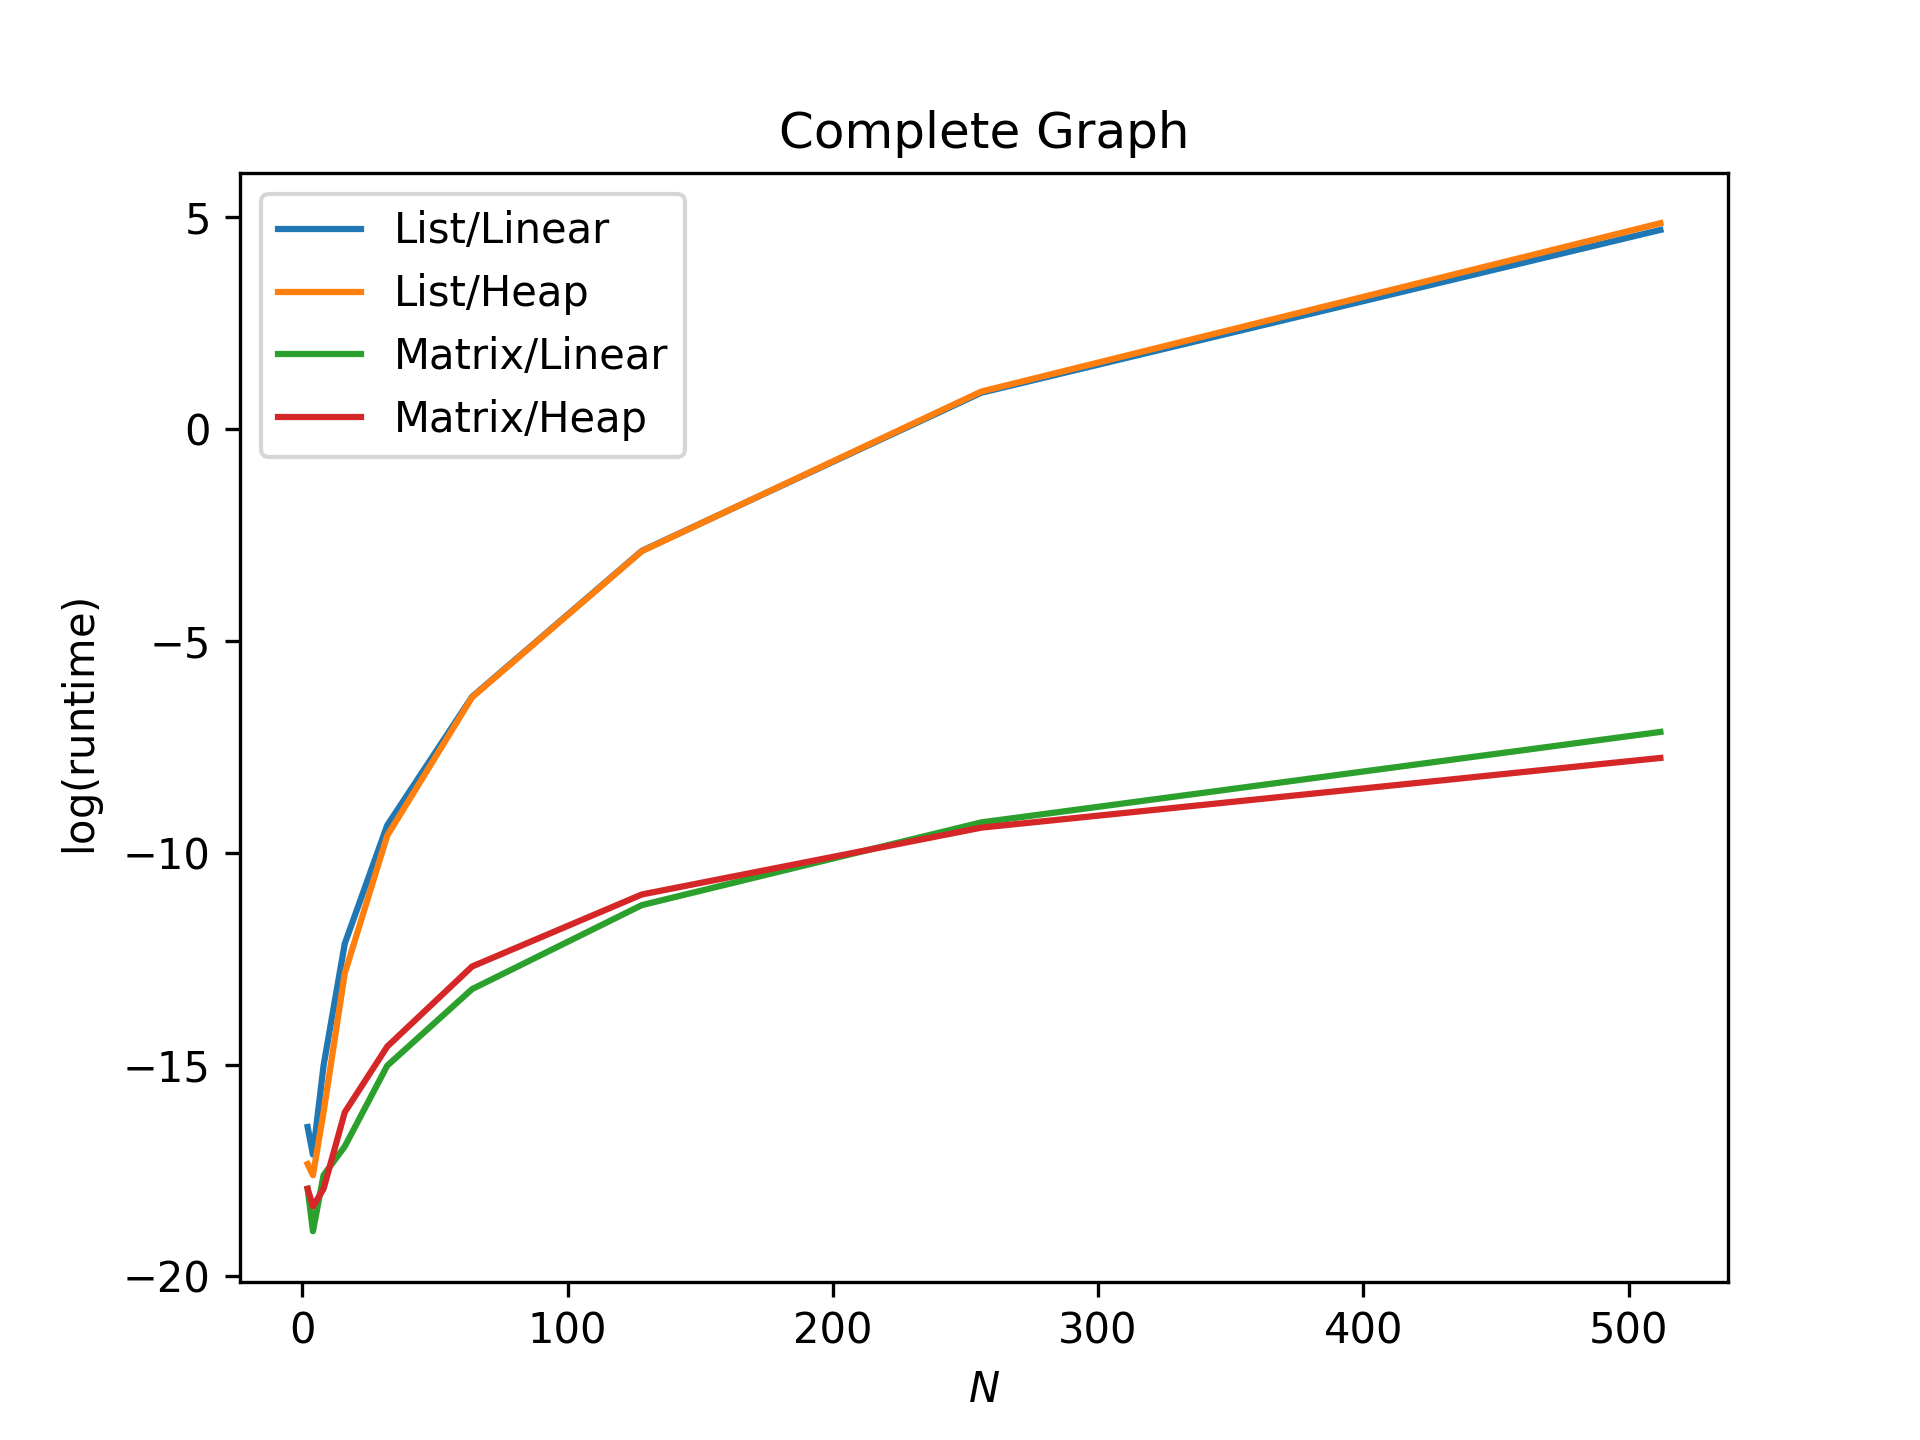
\includegraphics[width=\columnwidth]{./figure0.png}}
    \subfloat[]{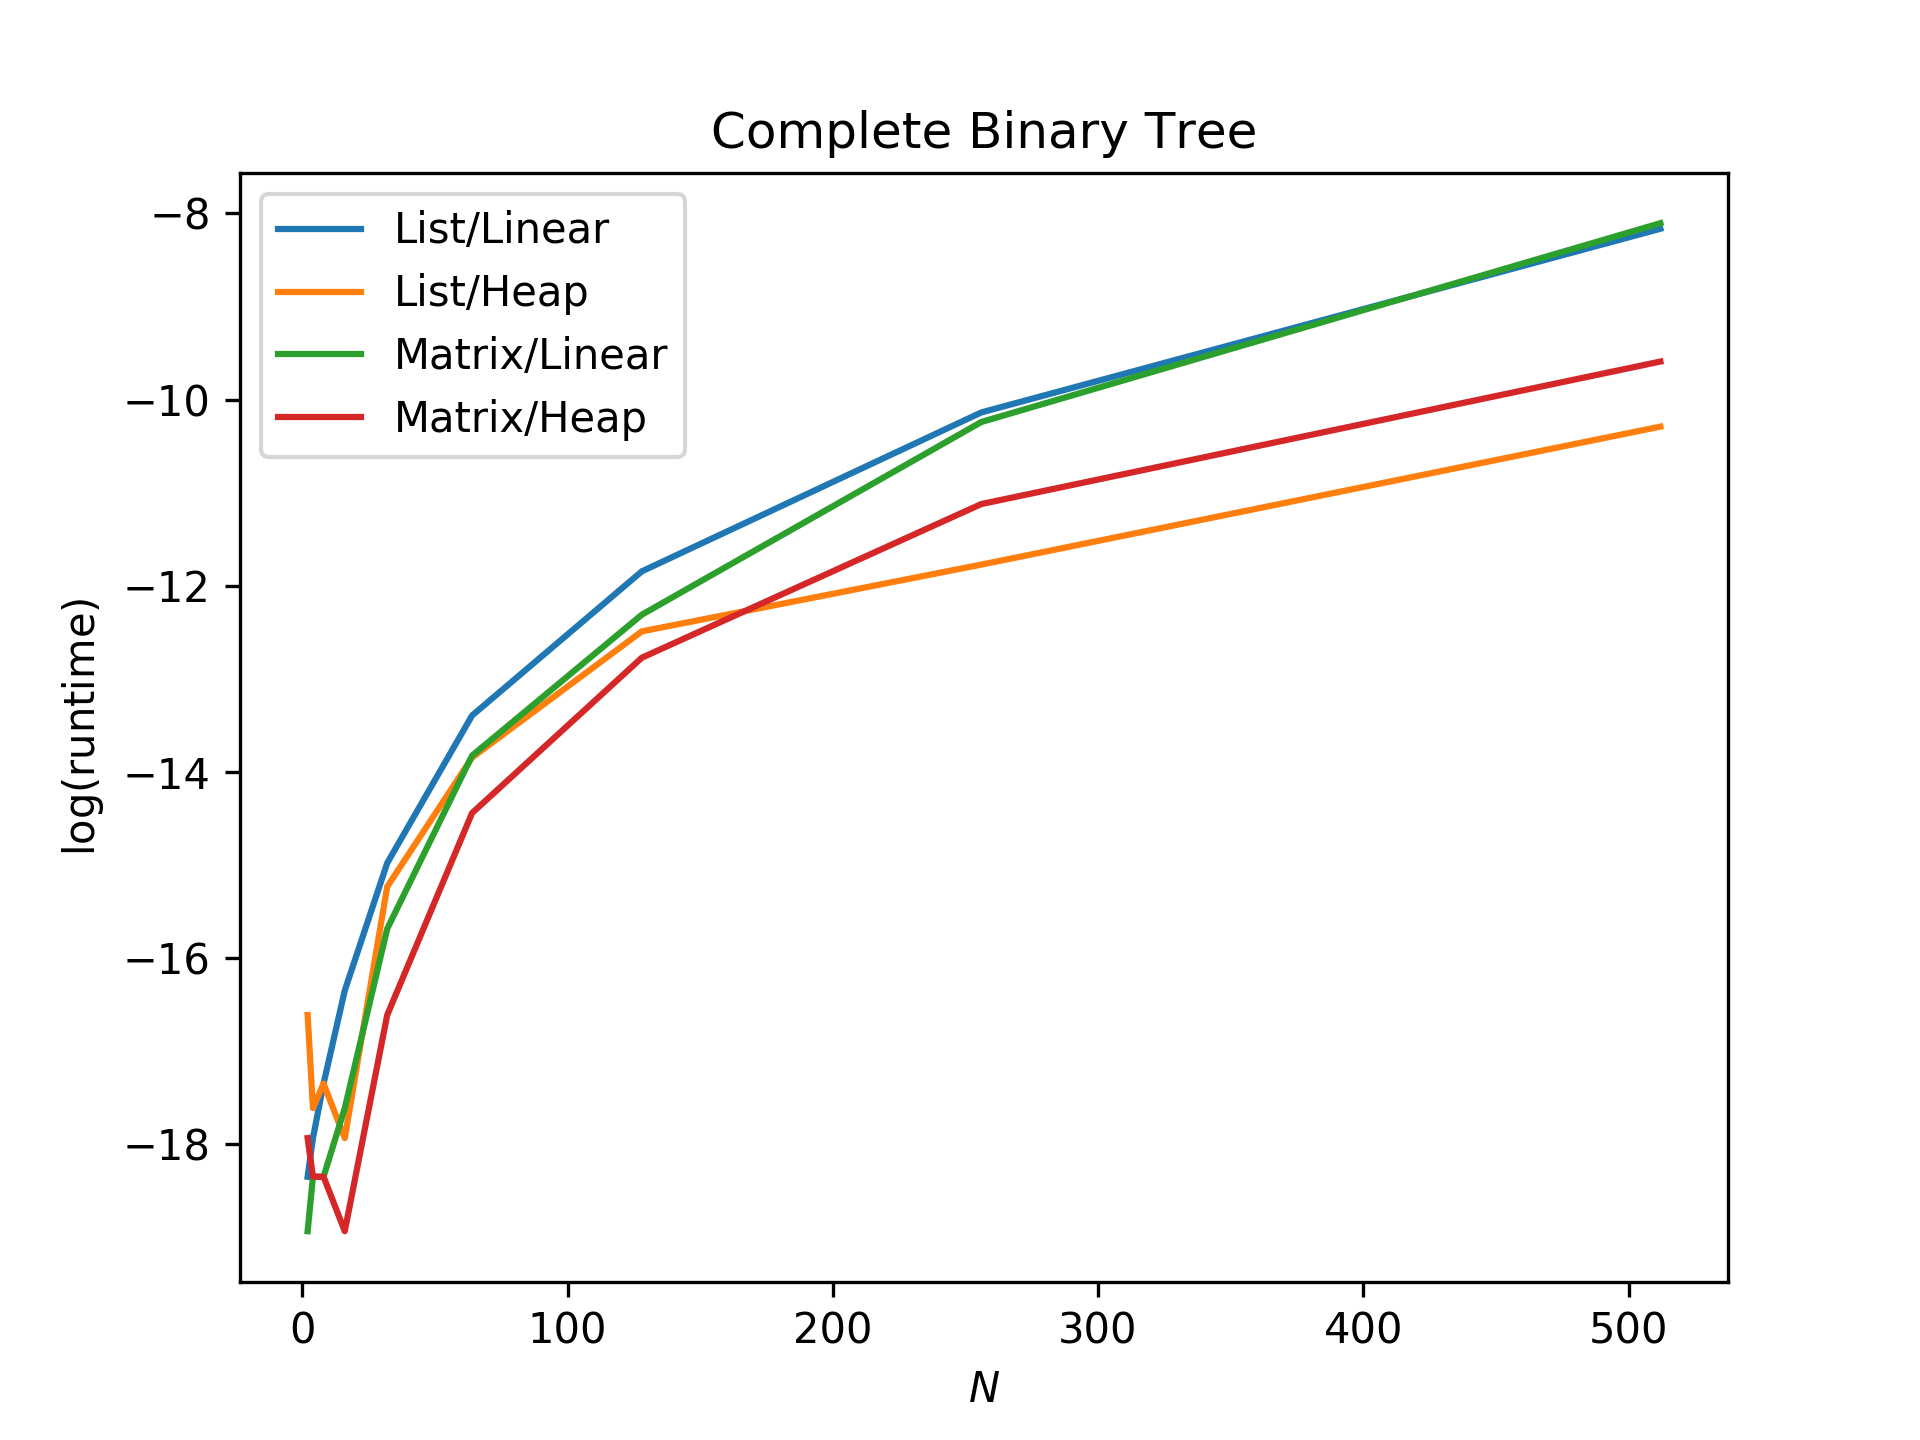
\includegraphics[width=\columnwidth]{./figure1.png}}

    \subfloat[]{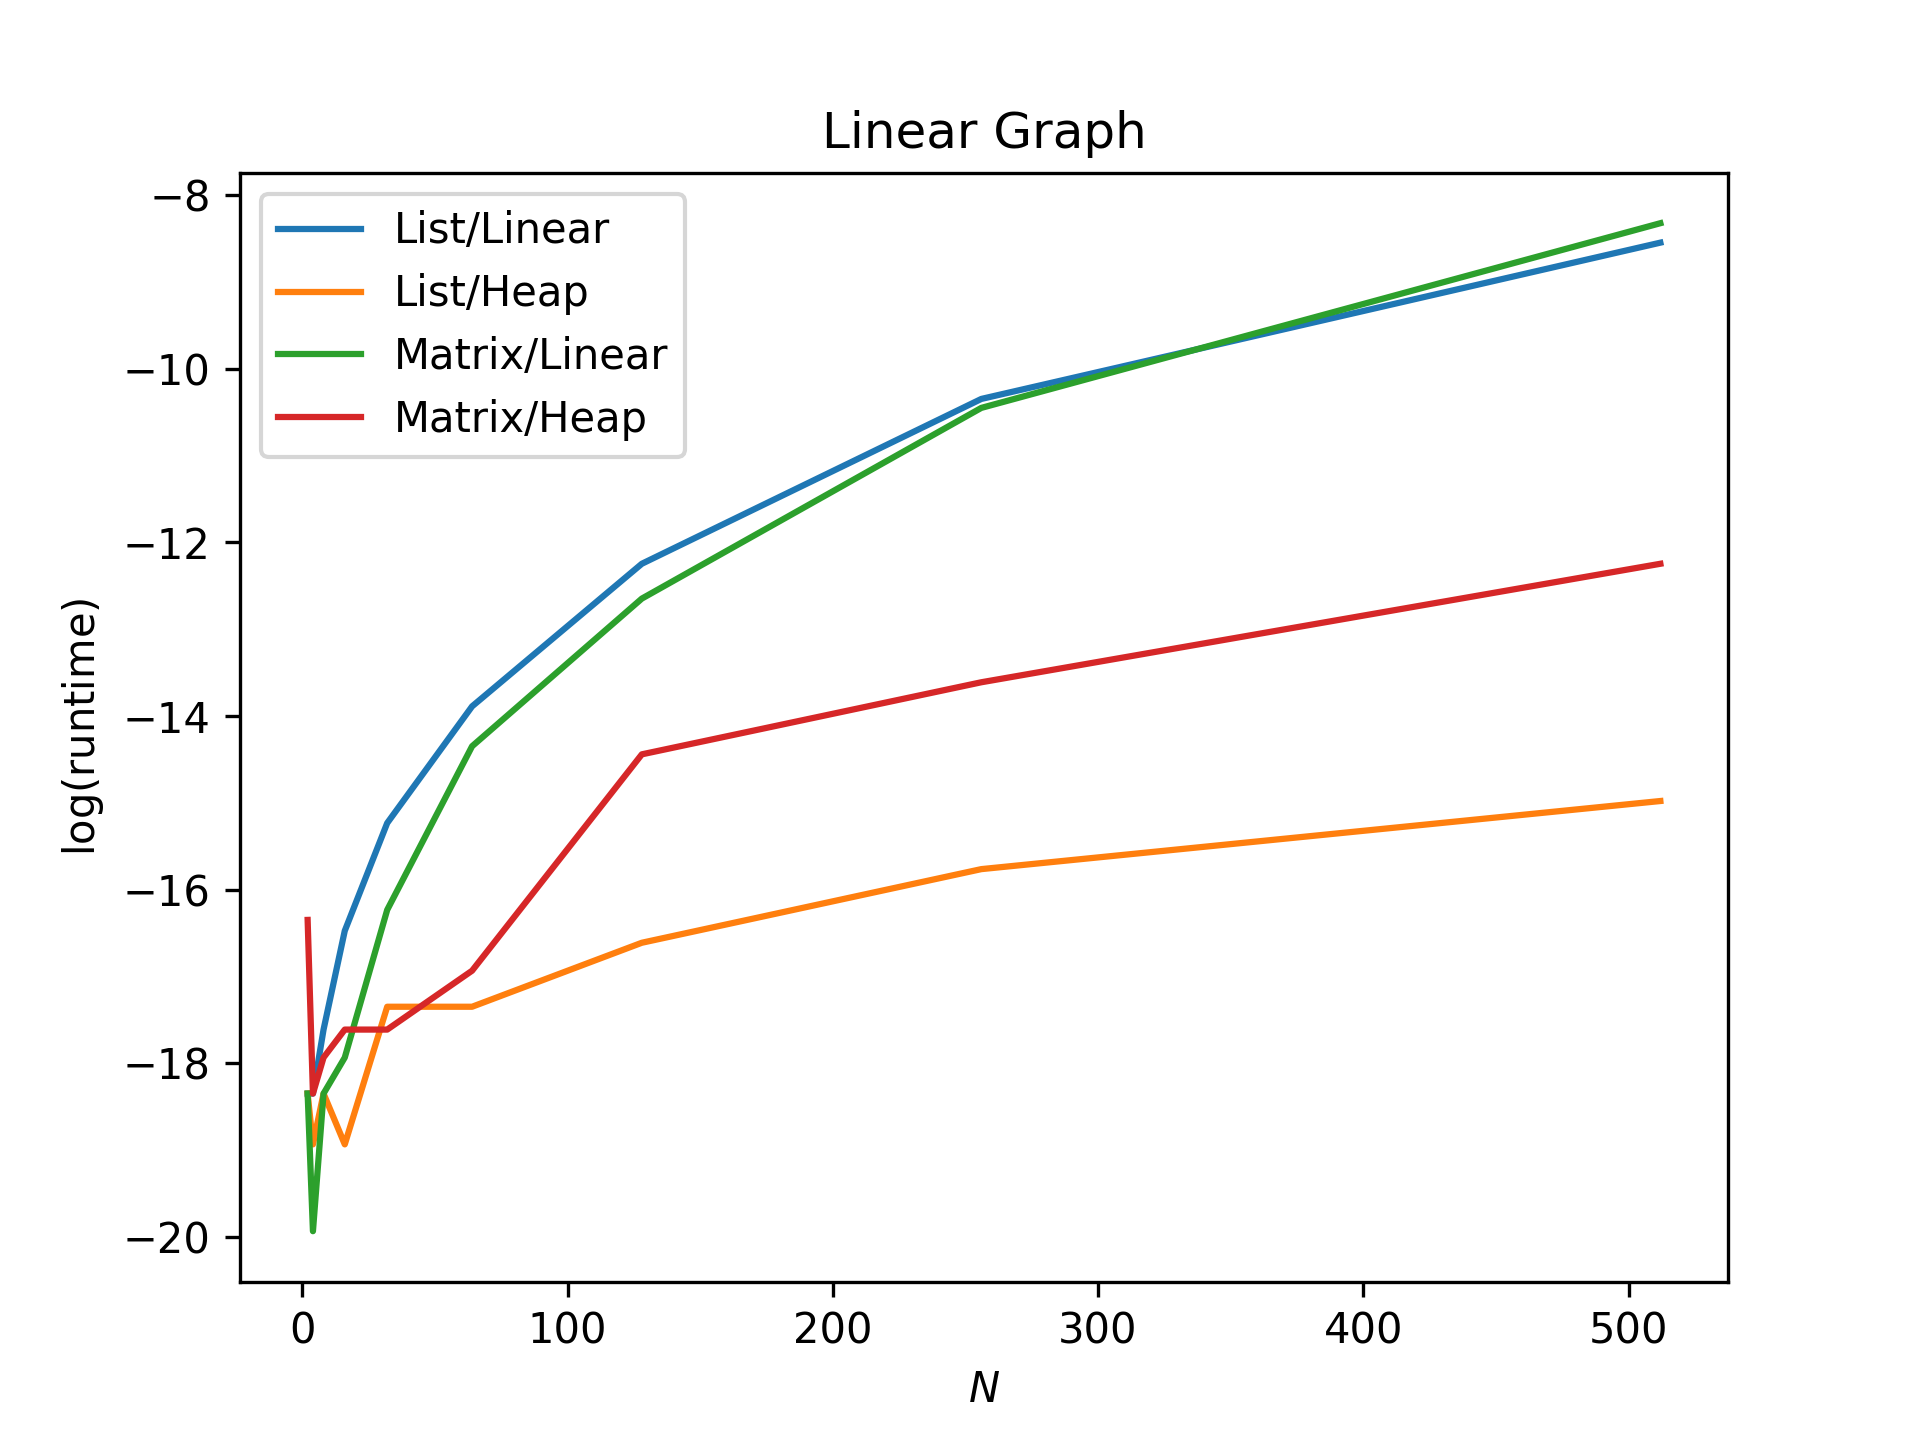
\includegraphics[width=\columnwidth]{./figure2.png}}
\end{figure*}


%\begin{table}[!ht]
    %\caption{Runtimes}
    %\centering
    %\begin{tabular}{|c|c|c|c|}
        %\hline
        %& DENSITY & LINEAR & HEAP \\ \hline
        %\multirow{3}{*}{Adjacency List} 
        %& Linear Graph & 0.0 & 0.0 \\ [0.5ex]\cline{2-4}
        %& Complete Binary Tree & 0.0 & 0.0 \\ \cline{2-4}
        %& Complete Graph & 0.0 & 0.0 \\ \hline
        %\multirow{3}{*}{Adjacency Matrix}
        %& & 0.0 & 0.0 \\ \cline{2-4}
        %& & 0.0 & 0.0 \\ \cline{2-4}
        %& & 0.0 & 0.0 \\ \hline
    %\end{tabular}
%\end{table}


\section{Conclusion}
Overall, our experimental results are consistent with our expectations.
For a complete graph of $N$ verticies, it seems regarding performance, 
the choice of graph representation takes precedent over the \texttt{minVertex} implementation.
For a complete binary tree, it seems that the heap implementation of 
\texttt{minVertex} yields higher performance, independent of 
the graph representation.
For a sparse graph, we see that the use of a heap in the 
\texttt{minVertex} function yields significantly higher peformance over 
the linear implementation. 

Thus, we can concluded that if $|E|$ is sufficiently smaller compared to 
$|V|$, then using a heap in \texttt{minVertex} becomes more efficient. 
Likewise, for very dense graphs, the use of linear \texttt{minVertex} 
yields significant improvements.

%{{{    Bibliography
\nocite{*}
\bibliographystyle{IEEEtran}
\bibliography{references.bib}
%}}}
\end{document}

